\documentclass[11pt, tikz]{standalone}
\usepackage[T1]{fontenc}
\usepackage[utf8]{inputenc}
%\usepackage{textcomp}
%\renewcommand{\ttdefault}{lmtt} % 
\usepackage{amsmath}
\usetikzlibrary{arrows.meta, decorations.pathmorphing, positioning, calc}
\usepackage{xcolor}

\usepackage{mwe,tikz}
\usepackage[percent]{overpic}
\pagestyle{empty}

\begin{document}\sffamily
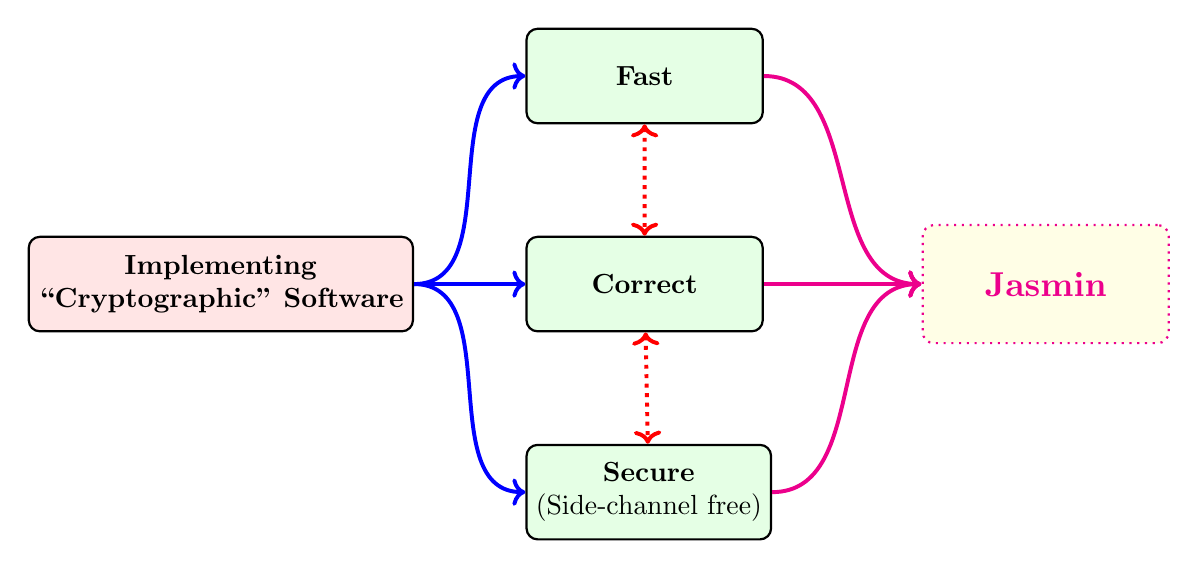
\begin{tikzpicture}[
	bluebox/.style={rectangle, draw, thick, rounded corners, minimum height=1.2cm, minimum width=2.5cm, align=center, fill=blue!10},
	yellowbox/.style={rectangle, draw, thick, rounded corners, minimum height=1.2cm, minimum width=2.5cm, align=center, fill=yellow!10},
	greenbox/.style={rectangle, draw, thick, rounded corners, minimum height=1.2cm, minimum width=3cm, align=center, fill=green!10},
	redbox/.style={rectangle, draw, thick, rounded corners, minimum height=1.2cm, minimum width=3cm, align=center, fill=red!10},
	arrow/.style={->, line width=.5mm},
	every node/.style={align=center}
	]
	
	%Draw Plaid
%	\draw[very thin,color=gray!15,step=.5] (-10,-5) grid (10,5);
%	%Take Coordinates
%	\foreach \i in {-4,...,-2,-1,1,2,...,4}
%	\draw[gray] (\i,.1)--(\i,-.1) node[below] {$\i$};%x-axis
%	\foreach \i in {-4,...,-2,-1,1,2,...,4}
%	\draw[gray] (.1,\i)--(-.1,\i) node[left] {$\i$};%y-axis
	
%	\node (fig1) at (0,0)
%	{\includegraphics[scale=0.5]{cryptographic-sw.pdf}};
%	\draw[dotted, purple] (-4,-2) rectangle (4,2);
%	\node[yellowbox,scale=.5] (jasmin) at (6,1.5) {Jasmin};
%	\draw[dotted, purple, -{Latex},out=0,in=180] (4,1.5) to (jasmin);
	
	
	\node[redbox] (crypto-sw) {\textbf{Implementing}\\ \textbf{``Cryptographic'' Software}};
	\node[greenbox, above right=2cm of crypto-sw] (ef) {\bfseries Fast};
	\node[greenbox, right=1.414cm of crypto-sw] (fc) {\bfseries Correct};
	\node[greenbox, below right=2cm of crypto-sw] (sca) {\bfseries Secure\\ (Side-channel free)};
	\draw[arrow, blue, out=0, in=180] (crypto-sw) to (ef);
	\draw[arrow, blue, out=0, in=180] (crypto-sw) to (sca);
	\draw[arrow, blue, out=0, in=180] (crypto-sw) to (fc);
	
	\draw[dotted, <->, line width=.5mm, red, out=-90, in=90] (ef) to (fc);
	\draw[dotted, <->, line width=.5mm, red] (fc) to (sca);
	
	\node[dotted, yellowbox, right=2cm of fc, draw=magenta, scale=1.25] (jasmin) {\bf\color{magenta} Jasmin};
	\draw[arrow, magenta, out=0, in=180] (ef) to (jasmin);
	\draw[arrow, magenta, out=0, in=180] (fc) to (jasmin);
	\draw[arrow, magenta, out=0, in=180] (sca) to (jasmin);
\end{tikzpicture}
\end{document}
